\documentclass[../document.tex]{subfiles}

\begin{document}
	\section{Эксперименты}
		\subsection{Сухогруз}
			\subsubsection{Scenario description}
				\begin{figure}[h]
					\centering
					\includegraphics[width=0.95\textwidth]{images/d1/bulker_setup.png}
					\caption{(color online) The measurements area and the noise monitoring stations, picture courtesy of Zizheng Li and Graham Warner (JASCO Applied Sciences).}
					\label{fig1:area}
				\end{figure}
				
%				\par In order to address these questions several workshops on sound propagation modelling have been organized recently, including a 2022 Cambridge Joint Industry Programme Acoustic Modelling (JAM) workshop \cite{ainslie_JAM_workshop,ainslie2019wsdub}. One of the model validation problems offered by the organizers to the participants was concerned with simulation of the noise produced by a bulk carrier vessel. In this scenario, the vessel is moving past an underwater listening station (ULS) deployed close to Saturna island near the Port of Vancouver \cite{macg_2022} (see Fig.~\ref{fig1:area}). The participants were provided with a the vessel track data (its transit of the closest point of approach  (CPA) to the monitoring station), the effective source level of an equivalent monopole, and the information on the environment including bathymetry in the area, historical sound speed profiles (SSP) for three months, and some limited data on the geoacoustic parameters of the bottom layers. The goal was to simulate the distribution of the sound levels over decidecade bands \cite{ainslie2022harmoniz,ainslie2021terminology} for various distances between the vessel and the monitoring station. The measurement data taken by the monitoring station were made available to the participants a posteriori for the validation of the modelling results.
				
				\par Одна из задач моделирования шума, создаваемого морским сухогрузом, была предложена в рамках Cambridge Joint Industry Programme Acoustic Modelling (JAM) workshop \cite{ainslie_JAM_workshop,ainslie2019wsdub}. В рамках данной задачи морское судно движется в пределах подводной станции акустического мониторинга, расположенной недалеко от острова Сатурна в порту Ванкувера \cite{macg_2022} (см. Рис. \ref{fig1:area}). В задаче известны траектория движения судна, эффективный спектр источника эквивалентного монополя, а также информация о среде, включающая батиметрию рассматриваемой области, исторические данные о профиле скорости звука за три месяца, и некоторые ограниченные данные о геоакустических параметрах донных слоёв. Задача состояла в моделировании уровней звука в децидекадных полосах \cite{ainslie2022harmoniz,ainslie2021terminology} на различных расстояниях от судна до станции мониторинга. Результаты измерений, полученных на станции мониторинга, также были получены для валидации результатов моделирования. 
				
%				\par The goal of the present study is to present the results of our work on this scenario and to share our understanding regarding the of the possible ways to improve the shipping noise modelling. The simulations in this study were carried out using the AMPLE code \cite{tyshchenko2021,ample} based on the mode parabolic equations technique \cite{jsv}. This method features the capability to perform full-wave modelling of sound propagation in the three-dimensional geoacoustic waveguide of a shallow sea. Thus, one of the key results of this work is an investigation of the role played by 3D effects in the shipping noise propagation. Although the propagation distances in the considered scenario are somewhat shorter than it is usually required for the 3D features of the sound field to develop, the strongly range-dependent environment in the narrow strait where the monitoring station was deployed favours the manifestation of the related effects. 
				
				\par Для решения данной задачи был применён комплекс программ AMPLE, разработанный в рамках данной работы (см. ГЛАВА), основанный на модовых параболических уравнениях (см. ЕЩЁ ГЛАВА). Использование такого метода обусловлено тем, что он позволяет проводить моделирование распространения звука с учётом трёхмерных особенностей волновода, что позволяет провести исследование трёхмерных эффектов распространения акустического шума, производимого морским судном.
				
%				\par In course of our work on the workshop scenario we discovered that it was impossible to achieve satisfactory agreement between the measurements and the simulation with the bottom parameters suggested by the organizers. To overcome this difficulty, we performed an optimization of the geoacoustic parameters aimed at achieving a better fit of the noise levels distribution at CPA, and afterwards the resulting measurement-adjusted bottom model was used for the modelling of noise for all positions of the vessel in the course of the CPA transit. We believe that such an optimization approach is practical when performing vessel noise monitoring in practice. 
				
				\par Во время работы над поставленной задачей было выяснено, что невозможно достичь удовлетворяемого согласия между измерительными данными и результатами моделирования с использованием параметров дна, представленными в задаче. Для преодоления этой проблемы была проведена оптимизация геоакустических параметров дна с целью достичь большего согласия распределения уровней шума в ближайшей точке приближения, и затем использовать полученные параметры модели дна при моделировании шума вдоль всего пути проходимого судном. Предполагается, что такой оптимизационный подход имеет практический смысл для применения в прикладных задачах.
				
%				\par Another challenge for the noise field simulation was related to the fact that we had a single reception point (i.e., the monitoring station) while the position of the source was slowly moving. Clearly, full 3D broadband modelling of the field for every source position is not feasible even with the most efficient codes. For this reason, we had to use the reciprocity principle \cite{jensen} and to compute the 3D acoustic field for all frequencies involved as if the source was located at the monitoring station. In this case the model can be run once for computing the noise levels along all points of the vessel track. This approach must be used with a due care when strong currents are present in the area of interest, and the equations of sound propagation must be adjusted in order to take the moving media effects into account.
%				At the same time, we expect it to produce acceptable results whenever the current velocity projection onto the source-receiver line is sufficiently small. 
				
				\par Другой трудностью, возникшей при проведении моделирования, является тот факт, что в задаче дана единственная точка приёма (то есть станция мониторинга), в то время как позиция источника постепенно изменяется. Очевидно, полное трёхмерное широкополосное моделирование звукового поля для каждой позиции источника является необозримой задачей даже для самых эффективных программ. В результате чего был использован принцип обратного взаимодействия \cite{jensen}, и трёхмерное акустическое поле было рассчитано для всех рассматриваемых частот. Таким образом, требуется лишь одно вычисления модели для получения уровней акустического шума вдоль всего пути судна. Использование данного подхода должно происходить с большой осторожностью, так как в том случае если в рассматриваемой области существуют сильные потоки, в уравнения распространения звука должны быть внесены поправки, чтобы учесть эффекты движения среды. В то же время, использованный метод должен показать приемлемые результаты, если проекция скорости движения среды на прямую источник-приёмник достаточно мала.
				
%				\par The paper is organized as follows: Section~\ref{sec:scenario} presents a brief scenario description. Section~\ref{sec:models} briefly describes the AMPLE sound propagation modelling tool, and the modelling results are discussed in Section~\ref{sec:results}, where noise distributions are computed both for original and for optimized media parameters. Key results, findings and observations are summarized in the Conclusion.

				\par КАК-ТО ОПИСАТЬ ЧТО БУДЕТ ДАЛЬШЕ?
				
				\par НАВЕРНОЕ НОВАЯ ГЛАВА?
				
%				\par As was mentioned in the Introduction the JAM workshop scenario under consideration corresponds to the transit of a bulk carrier vessel past a hydrophone system deployed in a strait near Saturna Island close to the Port of Vancouver. The vessel transiting past the hydrophones of a measurement system was tracked via the Automated Identification System (AIS). Source level data provided to the workshop participants were generated by an automated system (JASCO PortListen) that computes vessel source levels within a data window defined by a $\pm 30^\circ$ azimuth angle centred from the CPA to the hydrophone.  Source levels from a single transit of a vessel of opportunity were analyzed on the basis of SPL versus distance measurements in decidecade frequency bands with centre frequencies from 10 Hz to 250 kHz. PortListen computed propagation loss from the hydrophone to the vessel CPA using a wave equation model, assuming a source depth equal to 70\% of the vessel draft at the time of measurement. Additional details regarding the automated source level analysis  performed by PortListen are provided in \cite{Hannay_Mouy_Li_2016}. For the workshop validation scenarios, model predictions were compared to mean-square pressure versus frequency, $p^2_{ddec}(f)$, and sound exposure versus frequency, $E_{p,ddec}(f)$, in decidecade bands, as measured on the underwater listening station using a temporal observation window of 1\ sec at distances of up to 3.3 km from the hydrophone. Acoustic quantities are as defined in \cite{ISO18405} \cite{ainslie2021terminology}.
				
				\par Как было сказано ранее, рассматривается задача сухогруза мимо системы гидрофонов, расположенных по прямой около острова Сатурна в порте Ванкувера. Траектория судна относительно гидрофонов была получена с использованием системы автоматической идентификации. Полученный спектр источника был сгенерирован автоматической системой (JASCO PortListen), которая вычисляет уровни эффективного точечного источника соответствующего судну, внутри окна задаваемого азимутальным углом в $\pm30^\circ$ относительно направления гидрофон-судно. Уровни источника, полученные в результате прохождения единственного судна были использованы для построения и последующего анализа зависимости SPL (Sound Pressure Level) от расстояния в децидекадных частотных полосах с центральными частотами в пределах от 10 Гц до 250 кГц. Системой PortListen были вычислены потери распространения от гидрофона до ближайшей точки приближения судна с использованием волнового уравнения, предполагая глубину источника равной 70\% осадки судна на момент измерений. Дополнительные детали, относящиеся к автоматическому анализу спектра источника, проводимому PortListen, могут быть найдены в  \cite{Hannay_Mouy_Li_2016}. При проведении валидации было проведено сравнение результатов моделирования с усредненным квадратом давления относительно частоты $p^2_{ddec}\pa{f}$, и также акустической экспозиции относительно частоты $E_{p,ddec}\pa{f}$ в децидекадных полосах, измеренных подводной станцией акустического моделирования с использованием окна наблюдений по времени равным 1 с. на расстояниях до 3.3 км. от гидрофона. Акустические величины описаны в \cite{ISO18405} \cite{ainslie2021terminology}.  
				
				\begin{figure}[h]
					\centering
					\includegraphics[width=0.95\textwidth]{images/d1/bath.pdf}
					\caption{(color online) Bathymetry chart in the monitoring area and the vessel track in the Cartesian coordinates with the $x$ axis aligned approximately along the track and the receiver position specified by R.}
					\label{fig2:bath1}
				\end{figure}
		
%				\par The bathymetry in the area of vessel transit is shown in Fig.~\ref{fig2:bath1} where we introduced a Cartesian coordinate system centered at the receiver location and with an $x$ axis aligned along the bulk carrier track. The bottom in the area consists of an upper sediment layer (which is formed by fine-grained sand) overlying a bedrock substrate (the values of the geoacoustic parameters of the bottom suggested by the workshop organizers are given in  Table~\ref{tbl:optimization_parameters}).
				
				\par Батиметрия области прохождения судна показана на Рис.~\ref{fig2:bath1}. Была введена прямоугольная система координат с центром в позиции приёмника и осью $x$ расположенной параллельно пути движения сухогруза. Дно в данной области состоит из верхнего слоя осадков (состоящих в основном из мелкого песка), расположенного над слоём коренной породы (значения геоакустических параметров дна, предложенные НЕПОНЯТНО КЕМ отображены в Таблице~\ref{tbl:optimization_parameters}).
		
%				\par The historical sound speed profiles (SSP) for the Salish Sea available to the workshop participants are presented in Fig.~\ref{fig3:ssp} (note that the measurements took place in November, but the SSP data for October and December was aslo provided).
%				\begin{figure}[h]
%					\centering
%					\includegraphics[width=0.5\textwidth]{images/d1/ssp.pdf}
%					\caption{(color online) Historical data on sound speed profiles in the area of interest. }
%					\label{fig3:ssp}
%				\end{figure}
%				The effective source spectrum of the bulk carrier is shown in Fig.~\ref{fig4:sspectrum}. Note that it corresponds to the source level of an equivalent monopole \cite{ISO18405} and no information on the source directivity was given in the problem statement. 
				
				\par Исторические профили скорости звука в море Селиш представлены на Рис.~\ref{fig3:ssp} (стоит отметить, что эксперимент проходил в Ноябре, но данные за Октябрь и Декабрь также были доступны).
				
				\begin{figure}[h]
					\centering
					\includegraphics[width=0.5\textwidth]{images/d1/ssp.pdf}
					\caption{(color online) Historical data on sound speed profiles in the area of interest. }
					\label{fig3:ssp}
				\end{figure}
				
				\par Эффективный спектр источника шума, создаваемого сухогрузом, показан на Рис.~\ref{fig4:spectrum}. Стоит отметить, что спектр соответствует уровню источника эквивалентного монополя \cite{ISO18405}, при этом не было известно никакой информации о направленности источника.
		
%				\par The goal of the CPA transit simulation was to reproduce acoustic energy distribution over decidecade frequency bands $E_{p,ddec}(f)$ defined as
%				\begin{equation}
%					E_{p,ddec}(f_c,d) = 2\int_{f_1}^{f_2} |P(f,d)|^2 df\,,
%				\end{equation}
%				where $f_c$ is the central frequency of the band $[f_1,f_2]$, $P(f,d)$ is the spectrum at the receiver computed for a time window of 1 sec for a given point of the CPA transit, and $d$ is the distance from the ship to the hydrophone of the measurement system. Another important quantity is $\bar{p^2}_{ddec}(f)$ at CPA computed by the formula
%				\begin{equation}
%					\bar{p^2}_{ddec}(f) = E_{p,ddec}(f_c,d_{CPA})/T\,,
%				\end{equation}
%				where $T$ is the temporal observation window (hereafter $T=1$ sec), and $d_{CPA}$ is the distance from the ship to the measurement system at CPA. As we use a normal-mode-based model AMPLE, we decided that our attention is restricted to the frequency band EC2 (8.91 Hz -- 891 Hz). It was requested that the modelling results are averaged over decidecade frequency bands.
				
				\par Целью моделирования являлось воспроизведение распределения акустической энергии по децидекадным частотным полосам $E_{p,ddec}\pa{f}$, определяемым как
				\begin{equation}
					E_{p,ddec}\pa{f_c,d} = 2\int_{f_1}^{f_2} |P\pa{f,d}|^2 df\,,
				\end{equation}
				где $f_c$ -- центральная частота полосы $\left[f_1,f_2\right]$, $P\pa{f,d}$ -- спектр, вычисленный в приёмнике во временном окне равном 1 секунде для заданной точки на пути движения сухогруза, и $d$ -- расстояние от судна до гидрофона измерительной системы. Другим важным значением является $\bar{p^2}_{ddec}\pa{f}$ в ближайшей точке прохода судна, вычисляемое по формуле
				\begin{equation}
					\bar{p^2}_{ddec}\pa{f} = \nicefrac{E_{p,ddec}\pa{f_c,d_{CPA}}}{T}\,,
				\end{equation}
				где $T$ -- размер временного окна (здесь и далее $T=1$ секунда), и $d_{CPA}$ -- расстояние от судна до измерительной системы в ближайшей точке прохода. Так как программа AMPLE использует модель, основанную на нормальных модах, были рассмотрены частоты, соответствующие полосе EC2 (8.91 Гц. -- 891 Гц.). Требовалось, чтобы результаты моделирования были усреднены по децидекадным частотным полосам.
		
				\begin{figure}[h]
					\centering
					\includegraphics[width=0.6\textwidth]{images/d1/source_loglog.pdf}
%					\caption{Decidecade band source level spectrum of the bulk carrier (re 1 $\mu$Pa$^2$ m$^2$) as measured at the closest point of approach to the underwater listening station. The assumed source depth was 6.2 m. The identity and particulars of the vessel were anonymized and not shared with workshop participants. The length of the vessel is approximately 185 m and the beam approximately 30 m.}
					\caption{Децидекадные полосы уровней спектра источника шума, производимого сухогрузом (отн. 1 $\mu$Pa$^2$ m$^2$)}, измеренного в ближайшей точке прохода подводной акустической станцией. Глубина источника считается равной 6.2 м. Модель и параметры сухогруза не известны. Длина и ширина судна равнялась приблизительно 185 м. и 30 м. соответственно. 
					\label{fig4:sspectrum}
				\end{figure}
			\subsubsection{Проведение эксперимента}
%				\par All computations were done on a regular rectangular grid $x\in\left[20,3320\right]\,,y\in\left[-1000,1000\right]$ with the steps sizes $\Delta x=1\,,\Delta y=0.125\,,$ for the computations in both positive and negative directions of $x$ axis from the source, $z_s=192.7$. A perfectly matched layer was used to truncate the computational domain in $y$ (see \cite{jsv} for the details on the domain truncation). Acoustic modes we computed using the CAMBALA library that utilizes a finite-difference discretization of the Sturm-Liouville problem \eqref{Spectral} (the actual computations were performed using the step size $\Delta z=0.1$ in $z$).
				
				\par Все вычисления были проведены на равномерной прямоугольной сетке $x\in\left[20,3320\right]\,,y\in\left[-1000,1000\right]$ с размерами шагов $\Delta x=1\,,\Delta y=0.125\,,$ для вычислений как в положительном, так и в отрицательном направлении оси $x$ от источника, $z_s=192.7$. Согласованный поглощающий слой был использован для искусственного ограничения вычислительной области вдоль оси $y$. Акустические моды были вычислены с использованием библиотеки CAMBALA, которая использует конечно-разностную дискретизацию задачи Штурма-Лиувилля \eqref{Spectral} (вычисления были проведены с использованием шага по глубине $\Delta z=0.1$).   
				
%				$20$ CPU processes were utilized during computation. The acoustic fields were output on a smaller regular grid $n_x=331\,,n_y=321\,,n_z=11$. $E_{p,ddec}(f)$ were then obtained using a Wolfram Mathematica script.
				
				\par Во время вычислений было использовано 20 потоков. Акустическое поле было выведено на более грубой сетке $n_x=331\,,n_y=321\,,n_z=11$. $E_{p,ddec}\pa{f}$ затем были получены с использованием скрипта на языке Wolfram Mathematica (Вольфрам математика).
				
				\begin{table}[h]
					\centering
					\begin{tabular}{|c|c|c|c|c|c|c|}
						\hline
						\multicolumn{3}{|c|}{\renewcommand{\arraystretch}{0.5}\begin{tabular}{@{}c@{}}Frequency range \\ $Hz$\end{tabular}} & \multirow{2}{*}{\renewcommand{\arraystretch}{0.5}\begin{tabular}{@{}c@{}}Substrate \\ thickness \\ $m$\end{tabular}} & \multirow{2}{*}{\renewcommand{\arraystretch}{0.5}\begin{tabular}{@{}c@{}}Number of \\ modes\end{tabular}} & \multirow{2}{*}{\renewcommand{\arraystretch}{0.5}\begin{tabular}{@{}c@{}}Comp. time \\ $min$\end{tabular}}\\
						\cline{1-3}
						$f_0$ & $f_1$ & $\Delta f$ & & &\\
						\hline
						8 & 24 & 1 & 1200 & 8 & 20\\
						\hline
						25 & 99 & 1 & 1200 & 28 & 220 \\
						\hline
						100 & 298 & 2 & 800 & 80 & 530 \\
						\hline
						300 & 892 & 4 & 600 & 160 & 1470 \\
						\hline
					\end{tabular}
					\caption{Media parameters used in the simulation for different frequency ranges.}
					\label{tab1:direct_comput}
				\end{table}
			\subsubsection{Результаты эксперимента}
%				\par As mentioned in the introduction, we used a reciprocity principle to perform the vessel noise simulation. More precisely, we set up the source at the depth of 192.7~m at $x=0, y=0$ (the actual location of the measurement system) and performed the computation of the sound pressure field for all frequencies from 8 Hz to 891 Hz in the area $-3.3\mbox{ km} \leq x\leq 3.3\mbox{ km}$, $1\mbox{ km} \leq y\leq 1\mbox{ km}$ at $z=6.2\mbox{ m}$ which is specified in the scenario description as the effective depth of the source (see Cartesian coordinates in Fig.~\ref{fig2:bath1}). In other words, it was more efficient to simulate the sound propagation from the receiver to the source (hereafter this is called reciprocal modelling) than vice versa (direct modelling). After computing the horizontal cross-section of the acoustic field for a given frequency, acoustic pressure values were interpolated onto all points of the vessel track.
				
				\par Для проведения моделирования распространения шума, создаваемого судном, был использован принцип взаимности. А именно, источник был расположен на глубине $129.7$ м. на $x=0,y=0$ (позиция, в которой на самом деле расположена система мониторинга) и было проведено вычисление поля акустического давления для всех частот из диапазона от 8 Гц. до 891 Гц. в области $-3.3\mbox{ км} \leq x\leq 3.3\mbox{ км}$, $1\mbox{ км} \leq y\leq 1\mbox{ км}$ at $z=6.2\mbox{ м}$, которая является эффективной глубиной источника шума (см. прямоугольную систему координат на Рис.~\ref{fig2:bath1}). Другими словами, более эффективным является моделирование распространения звука от приёмника к источнику (здесь и далее это называется взаимным моделированием) нежели наоборот (прямое моделирование). После вычисления горизонтальных срезов акустического поля для каждой частоты, значения акустического давления были интерполированы на все точки пути движения судна.  
				
%				\par It was originally suggested by the organizers that the environment should be considered range-independent (i.e., homogeneous in $x,y$). Indeed, such simplification could be reasonable for distances of about $3-4\mbox{ km}$ for which horizontal refraction effects are usually insignificant. We decided, however, that it is interesting to evaluate the significance of these effects in this scenario. Thus, all computations were preformed both using a full 3D AMPLE code (in which the pseudodifferential parabolic equations were solved both in positive and negative directions of the $x$ axis) and its simple 2D counterpart (which is computationally cheaper by approximately a factor of $400$).
				
				\par Изначально авторами сценария было предложено считать параметры среды независящими от расстояния (то есть однородными по $x,y$). Действительно, такое упрощения может быть приемлемо для расстояний порядка $3-4\mbox{ км}$, для которых эффекты горизонтальной рефракции обычно считаются пренебрежимыми. Было решено, однако, что исследование степени влияния таких эффектов на результаты моделирования является интересной задаче в контексте данного сценария. Таким образом, все вычисления были проведены как с использованием полностью трёхмерного комплекса программ AMPLE (для которого псевдодифференциальные параболические уравнения были решены в обоих направлениях: положительном и отрицательном по оси $x$), так и с использованием простого двумерного аналога (для которого вычисления являются значительно более дешёвыми в приблизительно $400$ раз). 
				
%				\par The first modelling results we obtained were rather discouraging. Even at the CPA the levels of the simulated noise substantially exceeded those obtained from the measurements data (see Fig.~\ref{fig5:CPA_comparison}). The difference is even more noticeable when comparing the noise levels for the CPA transit on a distance-frequency diagram as shown in Fig.~\ref{fig6:noise_ddec_non_opt}. Although partly higher levels in the simulated field can be explained by the fact that AMPLE program does not take bottom elasticity into account (which typically results in higher transmission loss), the discrepancy is too large to be explained exclusively by this factor. Other possible explanations of this disagreement include an inaccuracy in the information on the geoacoustic parameters of the bottom, a disagreement between the actual hydrological conditions on the measurement day with the historical SSP data, and inadequate representation of large source as an infinitesimal monopole (i.e., the far-field approximation). While little can be done to properly correct the source directivity pattern both in the vertical and the horizontal plane without undertaking additional measurements, media parameters can be adjusted using the existing data. 
				
				\par Результаты первых вычислений оказались скорее неудовлетворительными. Даже в точке ближайшего прохода, уровни шума, полученные в результате моделирования, существенно превышали результаты измерений (см. Рис.~\ref{fig5:CPA_comparison}). Разнится становится ещё более заметной при сравнении уровней шума на графике по расстоянию и частоте, как показано на Рис.~\ref{fig6:noise_ddec_non_opt}. Не смотря на то, что высокие уровни в смоделированном поле могут быть частично объяснены тем, что программа AMPLE не учитывает упругость дна (что в большинстве случаев показывает увеличение потерь распространения), наблюдаемая разность является слишком большой, чтобы она могла быть объяснима лишь этим эффектом. Другими возможными объяснениями такого эффекта могут быть неточность информации об геоакустических параметрах дна, несогласованность между фактическими гидрологическими параметрами на момент проведения измерений и историческими данными профилей скорости звука, и неподходящее представления большого источника шума в виде бесконечного малого монополя (то есть аппроксимация в дальнем поле). В то время как невозможно провести правильную корректировку вида направленности источника как в вертикальной, так и в горизонтальной плоскости, без проведения дополнительных измерений, параметры среды могут быть изменены из уже имеющихся данных. 
				
				\begin{figure}[h]
					\centering
					\includegraphics[width=0.6\textwidth]{images/d1/compare.pdf}
%					\caption{(color online) Noise distribution over frequencies at CPA of the vessel transit track obtained from measurements data (solid line), and from the modelling results using the default (dashed line) and the optimized (dash-dot line) values of environment parameters.}
					\caption{Распределение шума по частотам в точке ближайшего прохода судна, полученное из данных измерений (сплошная линия), и из результатов моделирования с использованием исходных (пунктирная линия) и оптимизированных (пунктирная линия с точками) значений параметров среды.}
					\label{fig5:CPA_comparison}
				\end{figure}
				
%				\par Note that higher intensity of the simulated the vessel noise as compared to the data can be (at least partly) explained by somewhat stronger acoustic contrast across the water-bottom interface and somewhat smaller attenuation in the sediment layer than in the actual environment.
				
				\par Стоит также упомянуть, что высокая интенсивность шума судна, полученного в результатах моделирования, по сравнению с данными (по крайней мере частично) может быть объяснена сильным акустическим контрастом поперёк интерфейса вода-дно и несколько меньшим чем в действительности затуханием в слое осадков.
				
				\begin{figure}[h]
					\centering
					\begin{subfigure}[t]{0.9\textwidth}
						\centering
						\includegraphics[width=\textwidth]{images/d1/target.pdf}
						\caption{Data}
					\end{subfigure}
					\begin{subfigure}[t]{0.9\textwidth}
						\centering
						\includegraphics[width=\textwidth]{images/d1/ample_non_optimized.pdf}
						\caption{Simulation}
					\end{subfigure}
%					\caption{(color online) Noise levels (in dB) for the CPA transit obtained from measurement data (a) and the 3D modelling using the parameters provided by the workshop organizers (b).}\label{fig6:noise_ddec_non_opt}
					\caption{Уровни шума (в Дб.) для прохождения судна, полученные из данных измерений (a) и результатов трёхмерного моделирования с использованием параметров, предложенных авторами сценария (b).\label{fig6:noise_ddec_non_opt}}
				\end{figure}
				
%				\par Some features of the field can be analyzed by considering its vertical cross-section (e.g., in $x,z$-plane) shown in Fig.~\ref{fig7:vertical_section}a for the frequency of 400 Hz (just as an example).
				
				\par Некоторые свойства поля могут быть проанализированы, рассматривая его вертикальные срезы (то есть в плоскости $x,z$), показанные на Рис.~\ref{fig7:vertical_section} для частоты в $400$ Гц (в качестве примера). 
				
				\begin{figure}[h]
					\centering
					\begin{subfigure}[t]{0.9\textwidth}
						\centering
						\includegraphics[width=\textwidth]{images/d1/cross_non_optimized_400.pdf}
						\caption{default parameters}
					\end{subfigure}
					\begin{subfigure}[t]{0.9\textwidth}
						\centering
						\includegraphics[width=\textwidth]{images/d1/cross_optimized_400.pdf}
						\caption{optimized parameters}
					\end{subfigure}
%					\caption{(color online) Vertical cross-section of acoustic field for $f=400\mbox{ Hz}$ (in dB re 1 m from the source) for the parameters from the scenario description (a) and for the optimized parameter values (b).}
					\caption{Вертикальный срез акустического поля для частоты $f=400\mbox{ Гц}$ (в Дб. отн. 1 м. от источника) с использованием параметров среды, предложенных авторами сценария (a) и их значений, полученных в результате оптимизации (b).\label{fig7:vertical_section}}
				\end{figure}
				
%				\par A typical feature of the interference pattern is that near the ocean surface the intensity maximum is located few hundred meters away in range from the source (obviously, exactly the same situation could be also observed in non-reciprocal computations). Such interference structure of the field results in the formation of sidelobes in the noise distribution in Fig.~\ref{fig6:noise_ddec_non_opt}(b), i.e., elongated features corresponding to high noise intensity areas aligned at an angle of roughly $\pi/4$ to the distance axis. Although similar features can be also found in Fig.~\ref{fig6:noise_ddec_non_opt}(a) after a careful examination (and in fact they are natural for the considered source and receiver depths), the respective noise intensity is significantly lower in the measurement data. 

				\par Типичной характеристикой интерференсной картины является то, что максимум интенсивности поля около поверхности океана расположен на расстоянии в несколько сотен метров от источника (конечно, точно такая же ситуация наблюдалась бы при проведения прямого моделирования). Такая интерференсная структура поля формирует боковые лепестки в распределении шума на Рис.~\ref{fig6:noise_ddec_non_opt} (b), то есть продолговатые признаки относящиеся к областям с высокой интенсивностью шума расположенные под углом в примерно $\nicefrac{\pi}{4}$ к оси расстояния. Не смотря на то, что похожие признаки могут быть найдены на Рис.~\ref{fig6:noise_ddec_non_opt}(a) в результате тщательного исследования (и, на самом деле, они являются естественными для рассматриваемых глубин источника и приёмника), соответствующая им интенсивность шума является существенно меньшей в данных измерений.
				
%				\par Arguably, this discrepancy can partly result from a non-trivial source directivity pattern, while, on the other hand, it can be somewhat mitigated by correcting media parameters (especially for lower frequencies that carry the majority of the source energy).
				
				\par Конечно, такое различение от части может быть результатом нетривиальной структуры направленности источника, которое с другой стороны, может быть несколько устранено корректировкой параметров среды (особенно для низких частот, которые переносят большую часть энергии источника). 
				
				  
			\subsubsection{Оптимизация параметров среды}
%				\par Since the agreement between the measurements data and the modelling results obtained using the suggested values of geoacoustic parameters was not acceptable, we decided to perform the optimization of the latter using the CPA levels (for the entire frequency band EC2) as a reference. 
				
				\par Так как не было достигнуто приемлемого согласования между данными измерений и результатами моделирования с использованием геоакустических параметров, предложенных авторами сценария, было решено провести их оптимизацию, используя данные в ближайшей точке прохода (для всей полосы частот EC2) в качестве опорного решения. 
				
%				\par The optimization was focused on adjusting bottom parameters, namely thickness, sound speed, density and attenuation of the sediment, as well as the sound speed of the substrate. Since differentiating through mode computation is impractical, non-gradient methods were considered. We used the bayesian optimization method \cite{garnett_bayesoptbook_2023}, which quickly explores the target function and finds a value close to the local maximum using only a small number of target function evaluations. The latter is especially important since mode computation takes a considerable amount of time. The Bayesian optimization algorithm can be summarized in the following way
%				\begin{enumerate}
%					\item Given a target function $f: \Theta\mapsto\mathbb{R}$ obtain a prior $p\pa{f|\theta\in\Theta}$, describing how the function is expected to behave with respect to $\theta$. Here $\Theta$ is the set of all possible combinations of the optimization parameters (i.e. all possible combinations of bottom parameters).
%					\item Observe $n\in\mathbb{N}$ target function values $y_i=f\pa{\theta_i}$ at randomly selected points $\left\{\theta_i\right\}_{i=1}^n$.
%					\item Obtain a posterior $p\pa{f|\theta_1,\dots,\theta_n,y_1,\dots,y_n}$.
%					\item For each $j=\overline{1,m}\,,m\in\mathbb{N}$ do
%					\begin{enumerate}
%						\item Obtain the next best guess $\theta_{n+j}$ by maximizing some acquisition function $q: \Theta\mapsto\mathbb{R}$ that assigns a score to potential guesses based on their perceived ability to benefit the optimization process at the current posterior $p\pa{f|\theta_1,\dots,\theta_{n+j-1},y_1,\dots,y_{n+j-1}}$.
%						\item Observe target function value at the newly obtained point $y_{n+j}=f\pa{\theta_{n+j}}$.
%						\item Update the posterior $p\pa{f|\theta_1,\dots,\theta_{n+j},y_1,\dots,y_{n+j}}$.
%					\end{enumerate}
%					\item Output the maximal value $y_i$ with its respective point $\theta_i$.
%				\end{enumerate}
				
				\par Оптимизация была ориентирована на изменение параметров дна, а именно толщину, скорость звука, плотность и затухание в слое осадков, а также скорость звука в корневой породе. Так как дифференцирование процесса вычисления мод является чрезмерно затратной операцией, были рассмотрены неградиентные методы оптимизации. Была использована байесовская оптимизация \cite{garnett_bayesoptbook_2023}, которая позволяет быстро исследовать целевую функцию и найти значение близкое к локальному максимуму, используя лишь небольшое количество вычислений целевой функции. Последнее является особенно важным, так как вычисление мод требует существенных временных затрат. Алгоритм байесовской оптимизации может быть кратко описан следующим образом
				\begin{enumerate}
					\item Для заданной целевой функции $f: \Theta\mapsto\mathbb{R}$ получить априорное распределение $p\pa{f|\theta\in\Theta}$, которое описывает ожидаемое поведение функции в зависимости от параметра $\theta$. Здесь $\Theta$ является множеством  всех возможных комбинаций оптимизируемых параметров (то есть все возможные комбинации параметров дна).
					\item Вычислить $n\in\mathbb{N}$ значений целевой функции $y_i=f\pa{\theta_i}$ в случайно выбранных точках $\left\{\theta_i\right\}_{i=1}^n$.
					\item Получить апостериорное распределение $p\pa{f|\theta_1,\dots,\theta_n,y_1,\dots,y_n}$.
					\item Для каждого $j=\overline{1,m}\,,m\in\mathbb{N}$ выполнить
					\begin{enumerate}
						\item Получить следующую лучшую точку $\theta_{n+j}$ путём максимизации некоторой функции оценки $q: \Theta\mapsto\mathbb{R}$, которая присваивает потенциальным точкам скор (score) основываясь на их предполагаемой возможности способствовать процессу оптимизации при текущем апостериорном распределении.
						\item Вычислить значение целевой функции в новой найденной точке $y_{n+j}=f\pa{\theta_{n+j}}$.
						\item Обновить апостериорное распределение $p\pa{f|\theta_1,\dots,\theta_{n+j},y_1,\dots,y_{n+j}}$.
					\end{enumerate}
					\item Выдать максимальное значение $y_{max}=\max\limits_{i=\overline{1,n+m}}y_i$ и соответствующую ему точку $\theta_{max}=\argmax\limits_{\theta_i,i=\overline{1,n+m}}y_i$ в качестве результата работы алгоритма.
				\end{enumerate}  
				
%				\par The most commonly used prior is that of a Gaussian process \cite{garnett_bayesoptbook_2023}. It takes the following form
%				\begin{equation}
%					\label{eq:prior}
%					\begin{bmatrix}
%						f\pa{\theta}\\
%						f\pa{\theta_1}\\
%						\vdots\\
%						f\pa{\theta_n}
%					\end{bmatrix}\sim
%					\mathcal{N}\pa{\mu,
%						\begin{bmatrix}
%							k\pa{\theta, \theta} & k\pa{\theta,\theta_1} & \dots & k\pa{\theta,\theta_n}\\
%							k\pa{\theta_1, \theta} & k\pa{\theta_1,\theta_1} & \dots & k\pa{\theta_1,\theta_n}\\
%							\vdots & \vdots & \ddots & \vdots\\
%							k\pa{\theta_n, \theta} & k\pa{\theta_n,\theta_1} & \dots & k\pa{\theta_n,\theta_n}
%						\end{bmatrix}
%					}
%				\end{equation}
%				which is a multivariate normal distribution with the mean $\mu$ and covariance matrix $\left\{k\pa{\theta_i,\theta_j}\right\}_{i,j}$, where $k: \Theta\times\Theta\mapsto\mathbb{R}$ is a so-called kernel or covariance function. The posterior distribution is then given by
%				\begin{gather}
%					p\pa{f\pa{\theta}|\theta_1,\dots,\theta_n,f\pa{\theta_1},\dots,f\pa{\theta_n}}\sim\mathcal{N}\pa{m,s^2}\nonumber\\
%					m=\left\{k\pa{\theta,\theta_i}\right\}_{i=1}^n\cdot\pa{\left\{k\pa{\theta_i,\theta_j}\right\}_{i,j=1}^n}^{-1}\cdot\left\{f\pa{\theta_i}\right\}_{i=1}^n\label{eq:posterior}\\
%					s^2=k\pa{\theta,\theta}-\left\{k\pa{\theta,\theta_i}\right\}_{i=1}^n\cdot\pa{\left\{k\pa{\theta_i,\theta_j}\right\}_{i,j=1}^n}^{-1}\cdot\left\{k\pa{\theta,\theta_i}\right\}_{i=1}^n\nonumber
%				\end{gather}
%				For this particular task in our study we used Mat\'ern kernel
%				\begin{equation}
%					k\pa{\theta_i, \theta_j}=\frac{1}{\Gamma\pa{\nu}^{\nu-1}}\pa{\frac{\sqrt{2\nu}}{l}d\pa{\theta_i, \theta_j}}^{\nu}K_\nu\pa{\frac{\sqrt{2\nu}}{l}d\pa{\theta_i, \theta_j}}\,,
%				\end{equation}
%				where $\nu,l\in\mathbb{R}$ are the kernel parameters, $d\pa{\cdot,\cdot}$ is the Euclidean distance, $K_\nu\pa{\cdot}$ is a modified Bessel function of the second kind and $\Gamma\pa{\cdot}$ is the gamma function. The parameter $\nu$ controls the smoothness of the resulting function (see Fig.~\ref{fig:metern_samples}) and $l$ is the length scale parameter.
%				\begin{figure}[h]
%					\centering
%					\includegraphics[width=0.9\textwidth]{images/d1/matern_samples.pdf}
%					\caption{(color online) The function $f\pa{\theta}$ sampled from a multivariate normal distribution \eqref{eq:prior} with zero mean and covariance matrix defined by the Mat\'ern kernel with different values for the parameter $\nu$. $f\pa{\theta}$ and $\theta$ are dimensionless and are plotted to show the impact of $\nu$.}
%					\label{fig:metern_samples}
%				\end{figure}
				
				\par Наиболее часто используемым априорным распределением является таковое из Гауссовского процесса \cite{garnett_bayesoptbook_2023}, которое принимает следующий вид
				\begin{equation}
					\label{eq:prior}
					\begin{bmatrix}
						f\pa{\theta}\\
						f\pa{\theta_1}\\
						\vdots\\
						f\pa{\theta_n}
					\end{bmatrix}\sim
					\mathcal{N}\pa{\mu,
						\begin{bmatrix}
							k\pa{\theta, \theta} & k\pa{\theta,\theta_1} & \dots & k\pa{\theta,\theta_n}\\
							k\pa{\theta_1, \theta} & k\pa{\theta_1,\theta_1} & \dots & k\pa{\theta_1,\theta_n}\\
							\vdots & \vdots & \ddots & \vdots\\
							k\pa{\theta_n, \theta} & k\pa{\theta_n,\theta_1} & \dots & k\pa{\theta_n,\theta_n}
						\end{bmatrix}
					}
				\end{equation}
				и в свою очередь является многомерным нормальным распределением со средним $\mu$ и матрицей ковариации  $\left\{k\pa{\theta_i,\theta_j}\right\}_{i,j}$, где $k: \Theta\times\Theta\mapsto\mathbb{R}$ является так называемым ядром или функцией ковариации. Таким образом апостериорное распределение может быть выражено как
				\begin{gather}
					p\pa{f\pa{\theta}|\theta_1,\dots,\theta_n,f\pa{\theta_1},\dots,f\pa{\theta_n}}\sim\mathcal{N}\pa{m,s^2}\nonumber\\
					m=\left\{k\pa{\theta,\theta_i}\right\}_{i=1}^n\cdot\pa{\left\{k\pa{\theta_i,\theta_j}\right\}_{i,j=1}^n}^{-1}\cdot\left\{f\pa{\theta_i}\right\}_{i=1}^n\label{eq:posterior}\\
					s^2=k\pa{\theta,\theta}-\left\{k\pa{\theta,\theta_i}\right\}_{i=1}^n\cdot\pa{\left\{k\pa{\theta_i,\theta_j}\right\}_{i,j=1}^n}^{-1}\cdot\left\{k\pa{\theta,\theta_i}\right\}_{i=1}^n\nonumber
				\end{gather}
				В рамках данной работы было использована функция ковариации Матерна
				\begin{equation}
					k\pa{\theta_i, \theta_j}=\frac{1}{\Gamma\pa{\nu}^{\nu-1}}\pa{\frac{\sqrt{2\nu}}{l}d\pa{\theta_i, \theta_j}}^{\nu}K_\nu\pa{\frac{\sqrt{2\nu}}{l}d\pa{\theta_i, \theta_j}}\,,
				\end{equation}
				где $\nu,l\in\mathbb{R}$ являются параметрами ядра, $d\pa{\cdot,\cdot}$ -- евклидово расстояние, $K_\nu\pa{\cdot}$ -- модифицированная функция Бесселя второго рода и $\Gamma\pa{\cdot}$ -- гамма функция. Параметр $\nu$ задаёт гладкость функции, получаемой из распределения (см. Рис.~\ref{fig:metern_samples}), а $l$ является параметром масштаба.
				
%				\par The value $\nu=\frac{5}{2}$ was used and the kernel is transformed to
%				\begin{equation}
%					k\pa{\theta_i, \theta_j}=\pa{1+\frac{\sqrt{5}}{l}d\pa{\theta_i, \theta_j}+\frac{5}{3l}d\pa{\theta_i, \theta_j}^2}\exp\pa{-\frac{\sqrt{5}}{l}d\pa{\theta_i, \theta_j}}\,.
%				\end{equation}
%				This value provides good balance between function smoothness and its ability to approximate coarse data and allows for computing the kernel without evaluating the modified Bessel function. The parameter $l$ is initially set to $1$ and gets updated during the optimization process to better fit the observed data.
				
				\par Было использовано значение $\nu=\frac{5}{2}$, при котором ядро преобразуется к следующему виду
				\begin{equation}
					k\pa{\theta_i, \theta_j}=\pa{1+\frac{\sqrt{5}}{l}d\pa{\theta_i, \theta_j}+\frac{5}{3l}d\pa{\theta_i, \theta_j}^2}\exp\pa{-\frac{\sqrt{5}}{l}d\pa{\theta_i, \theta_j}}\,.
				\end{equation}
				Такое значение показывает хороший баланс между гладкостью функции и её возможность аппроксимировать шероховатые данные, а также позволяет провести вычисление ядра без необходимости оценивать значение функции Бесселя. Параметр $l$ изначально считается равным $1$, и затем обновляется в процессе обучения с целью более точно аппроксимировать наблюдаемые данные. 
				
%				\par For the acquisition function Upper Confidence Bound was used
%				\begin{equation}
%					q\pa{\theta}=\operatorname{E}\left[X_\theta\right]+\kappa\sqrt{\operatorname{Var}\pa{X_\theta}}\,,
%				\end{equation}
%				where $X_\theta\sim\mathcal{N}\pa{m,s^2}$ is a random variable distributed according to the posterior distribution \eqref{eq:posterior}. The parameter $\kappa\in\mathbb{R}$ controls the balance of exploitation and exploration with lower values promoting points around the target function peaks and higher values allow points to be selected from the whole range (see Fig.~\ref{fig:ucb}).
%				\begin{figure}
%					\centering
%					\includegraphics[width=0.9\textwidth]{images/d1/ucb.pdf}
%					\caption{(color online) Points selected during Bayesian optimization using Upper Confidence Bound acquisition function with different values for parameter $\kappa$. $f\pa{\theta}$ is an arbitrary function the optimization was performed for to show the impact of $\kappa$.}
%					\label{fig:ucb}
%				\end{figure}
		
				\par В качестве функции оценки была использована так называемая верхняя граница уверенности
				\begin{equation}
					q\pa{\theta}=\operatorname{E}\left[X_\theta\right]+\kappa\sqrt{\operatorname{Var}\pa{X_\theta}}\,,
				\end{equation}
				где $X_\theta\sim\mathcal{N}\pa{m,s^2}$ является случайной переменной распределённой согласно апостериорному распределению \eqref{eq:posterior}. Параметр $\kappa\in\mathbb{R}$ задаёт баланс между эксплуатацией и исследованием, при этом для маленьких значений параметра предпочитаются точки, находящиеся около локальных максимумов функции, а большие значения позволяют точкам быть выбранным из всего диапазона (см. Рис.~\ref{fig:ucb}).
				
%				\par The optimization was performed in Python using BayesianOptimization library \cite{bayesian_optimzation_lib}. To facilitate the process, the mode computation was re-implemented using Tensorflow library \cite{tensorflow2015-whitepaper} which allows the computations to be performed on a GPU and decreases the time it takes to obtain CPA levels for the entire frequency range from several hours to several minutes.
				
				\par Оптимизация была выполнена на языке Python с использованием пакета BayesianOptimization \cite{bayesian_optimzation_lib}(Байесовская оптимизация). Для ускорения процесса, вычисление мод было переписано с использованием библиотеки Tensorflow \cite{tensorflow2015-whitepaper}, которая позволяет проводить вычисления на графическом процессоре и таким образом уменьшает время, затрачиваемое на получение уровней в ближайшей точке прохода для всего набора частот, с нескольких часов до нескольких минут.
				
%				\par For the target function the negative mean squared difference between logarithms of the noise level at CPA obtained from measurements data and from the modeling results was used
%				\begin{equation}
%					f\pa{\theta}=-\frac{1}{N_F}\sum\limits_{f_c}\pa{\log{\pa{E_{p,ddec}\pa{f_c, d_{CPA}}}}-\log{\pa{E_{p,ddec}^{mod}\pa{f_c, d_{CPA},\theta}}}}^2\,,
%				\end{equation}
%				where $N_F$ is number of decidecade bands taken into account, $E_{p,ddec}^{mod}\pa{f_c,d_{CPA},\theta}$ is the modeling result for central frequency $f_c$, distance $d_{CPA}$ and media parameters $\theta$.
				
				\par В качестве целевой функции был использован средний квадрат разности логарифмов уровней шума в ближайшей точке прохода, полученные из данных измерений и результатов моделирования
				\begin{equation}
					f\pa{\theta}=-\frac{1}{N_F}\sum\limits_{f_c}\pa{\log{\pa{E_{p,ddec}\pa{f_c, d_{CPA}}}}-\log{\pa{E_{p,ddec}^{mod}\pa{f_c, d_{CPA},\theta}}}}^2\,,
				\end{equation}
				где $N_F$ -- количество рассматриваемых децидекадных полос, а $E_{p,ddec}^{mod}\pa{f_c,d_{CPA},\theta}$ результат моделирования для центральной частоты $f_c$, расстояния $d_{CPA}$ и параметров среды $\theta$.
				
%				\par The sound speed profile in the water column was also adjusted in course of the optimization. It was parameterized by a scalar parameter $t\in\left[-1,1\right]$ as an argument of a function linearly interpolated \textcolor{blue}{depth-by-depth} between the three nodes $-1\,,0\,,1$. \textcolor{blue}{The interpolation function can be expressed as follows}
%				\begin{equation}
%					c_{water}\pa{z,t}=\begin{cases}
%							c_{oct}\pa{z}+\pa{t+1}\pa{c_{nov}\pa{z}-c_{oct}\pa{z}}\,, & -1\leq t\leq 0\,,\\
%							c_{nov}\pa{z}+t\pa{c_{dec}\pa{z}-c_{nov}\pa{z}}\,, & 0<t\leq 1\,,
%					\end{cases}
%				\end{equation}
%				\textcolor{blue}{where $c_{oct},c_{nov},c_{dec}$ are the sound speed profiles for October, November, and December, respectively (see Fig.~\ref{fig3:ssp}).}
				
				\par Профиль скорости звука в воде также был рассмотрен во время проведения оптимизации. Он был параметризован единственным скалярным параметром $t\in\left[-1,1\right]$ как аргументом функции линейно интерполированной для каждой глубины между тремя узлами $-1\,,0\,,1$. Интерполированная функция может быть выражена как
				\begin{equation}
					c_{water}\pa{z,t}=\begin{cases}
						c_{oct}\pa{z}+\pa{t+1}\pa{c_{nov}\pa{z}-c_{oct}\pa{z}}\,, & -1\leq t\leq 0\,,\\
						c_{nov}\pa{z}+t\pa{c_{dec}\pa{z}-c_{nov}\pa{z}}\,, & 0<t\leq 1\,,
					\end{cases}
				\end{equation}
				где $c_{oct},c_{nov},c_{dec}$ -- профили скорости звука в воде за Октябрь, Ноябрь и Декабрь соответственно (см. Рис.~\ref{fig3:ssp}).
				
%				\par \textcolor{blue}{The sound speed for the sediment bottom layer is parameterized as follows}
%				\begin{equation}
%					c_{sediment}\pa{z}=c+\frac{z-z_b}{\Delta z}\Delta c\,,
%				\end{equation}
%				\textcolor{blue}{where $z_b$ is the bottom depth, $\Delta z$ is the sediment layer thickness, $c$ is the sound speed at the top of the layer, and $\Delta c$ is the sound speed difference.}
				
				\par Скорость звука в слое осадков была параметризирована следующим образом
				\begin{equation}
					c_{sediment}\pa{z}=c+\frac{z-z_b}{\Delta z}\Delta c\,,
				\end{equation}
				где $z_b$ -- глубина дна, $\Delta z$ -- толщина слоя осадков, $c$ скорость звука на вершине слоя, и $\Delta c$ разница в скорости звука.
				
%				\par The optimization parameter ranges and their values obtained during the optimization process are shown in Table.~\ref{tbl:optimization_parameters}. Note that the best agreement of the sound levels at CPA is achieved for October sound speed data and for somewhat lower sound speed in the upper part of the sediment layer that suggested by the workshop organizers. Optimization also results in a much higher sediment attenuation parameter that one might normally expect. This can be explained by the fact that the models we used do not take elasticity effects into account. Since the presence of shear waves in the bottom results in additional loss of acoustic energy, an unrealistically large value of attenuation in an equivalent fluid bottom model must compensate for it. Also note that the best model-data fit is achieved for the maximum sediment density value in the search interval. This can be explained by the low sensitivity to this parameter that is quite common for geoacoustic inversion problems. We decided not to extend this interval any further in order to keep this value reasonable. The quality of the optimization results can be assessed by comparing the sound level plots in Fig.~\ref{fig5:CPA_comparison}.
				
				\par Диапазоны оптимизируемых параметров и их значения, полученные в результате оптимизации показаны в Таб. ~\ref{tbl:optimization_parameters}. Стоит заметить, что наибольшее согласия уровней шума в ближайшей точке прохода было достигнуто для профиля скорости звука за Октябрь с несколько меньшей скоростью звука в слое осадков по сравнению с параметрами, предложенными авторами сценария. В результате оптимизации также были получены значительно большие значения параметра затухания, чем можно было бы ожидать. Это может быть объяснено тем, что используемые модели не учитывают эффекты упругости. Наличие поперечных волн в дне вносит дополнительную потерю акустической энергии, в результате чего неожиданно большое значение затухания в эквивалентной модели жидкого дна должен компенсировать этот эффект. Также стоит заметить, что наилучшее согласие модели и данных было достигнуто при максимальном значение плотности слоя осадков в рассматриваемом интервале. Это может быть объяснено низкой чувствительностью модели к данному параметру, что часто возникает в задачах геоакустической инверсии. Было решено не увеличивать интервал больше с целью удержать этот параметр в разумных пределах. Качество результатов оптимизации может быть оценено из графиков уровней шума на Рис.~\ref{fig5:CPA_comparison}.
				
				\begin{figure}[h]
					\centering
					\begin{subfigure}[t]{0.9\textwidth}
						\centering
						\includegraphics[width=\textwidth]{images/d1/ample_epddec.pdf}
						\caption{AMPLE, 3D}
					\end{subfigure}
					\begin{subfigure}[t]{0.9\textwidth}
						\centering
						\includegraphics[width=\textwidth]{images/d1/flat_epddec.pdf}
						\caption{2D}
					\end{subfigure}
					\begin{subfigure}[t]{0.9\textwidth}
						\centering
						\includegraphics[width=\textwidth]{images/d1/flat_ample_difference.pdf}
						\caption{Difference}
					\end{subfigure}
					\caption{(color online) Vessel sound level (in dB) simulated for the CPA transit with the optimized environment parameters.}\label{fig8:noise_ddec_opt}
				\end{figure}
				
				\begin{figure}[h]
					\centering
					\begin{subfigure}[t]{0.9\textwidth}
						\centering
						\includegraphics[width=\textwidth]{images/d1/field_optimized_100.pdf}
						\caption{100 Hz}
					\end{subfigure}
					\begin{subfigure}[t]{0.9\textwidth}
						\centering
						\includegraphics[width=\textwidth]{images/d1/field_optimized_200.pdf}
						\caption{200 Hz}
					\end{subfigure}
					\begin{subfigure}[t]{0.9\textwidth}
						\centering
						\includegraphics[width=\textwidth]{images/d1/field_optimized_400.pdf}
						\caption{400 Hz}
					\end{subfigure}
					\caption{(color online) Horizontal cross-sections of acoustic field (in dB re 1 m) at individual frequencies obtained as a solution of Eq.~\eqref{eq:helmholtz} (see supplementary material for an animation showing all frequencies). Isobaths in the area are shown by solid black lines.}\label{fig10:indiv_freqs}
				\end{figure}
				
				\begin{figure}[h]
					\centering
					\begin{subfigure}[t]{0.9\textwidth}
						\centering
						\includegraphics[width=\textwidth]{images/d1/optimzied_20.pdf}
						\caption{optimized parameters}
					\end{subfigure}
					\begin{subfigure}[t]{0.9\textwidth}
						\centering
						\includegraphics[width=\textwidth]{images/d1/non_optimzied_20.pdf}
						\caption{default parameters}
					\end{subfigure}
					\caption{(color online) Accuracy of the bulk carrier sound simulation (in dB) for the CPA transit with the optimized media parameters (a) and the parameters suggested in the scenario description (b).}\label{fig9:accuracy}
				\end{figure}
				
				\begin{table}[h]
					\centering
					\begin{tabular}{|c|c|c|c|c|c|c|c|c|c|}
						\hline
						\multirow{3}{*}{} & \multicolumn{5}{c|}{Sediment} & \multicolumn{3}{c|}{Substrate} & \multirow{3}{*}{SSP}\\
						\cline{2-9}
						&
						\multirow{2}{*}{\renewcommand{\arraystretch}{0.5}\begin{tabular}{@{}c@{}}Thickness \\ $\Delta z, m$\end{tabular}} &
						\multicolumn{2}{c|}{\renewcommand{\arraystretch}{0.5}\begin{tabular}{@{}c@{}}Sound speed \\ $m/s$\end{tabular}} &
						\multirow{2}{*}{\renewcommand{\arraystretch}{0.5}\begin{tabular}{@{}c@{}}Density \\ $g/cm^3$\end{tabular}} &
						\multirow{2}{*}{\renewcommand{\arraystretch}{0.5}\begin{tabular}{@{}c@{}}Attenuation \\ $dB/\lambda$\end{tabular}} &
						\multirow{2}{*}{\renewcommand{\arraystretch}{0.5}\begin{tabular}{@{}c@{}}Sound speed \\ $m/s$\end{tabular}} &
						\multirow{2}{*}{\renewcommand{\arraystretch}{0.5}\begin{tabular}{@{}c@{}}Density \\ $g/cm^3$\end{tabular}} &
						\multirow{2}{*}{\renewcommand{\arraystretch}{0.5}\begin{tabular}{@{}c@{}}Attenuation \\ $dB/\lambda$\end{tabular}}&\\
						\cline{3-4}
						& & $c$ & $\Delta c$ & & & & & &\\
						\hline
						default & $50$ & $1541$ & $50$ & $1.8$ & $0.61$ & $2160$ & $2$ & $0.25$ & 0\\
						\hline
						optimized & $61.4$ & $1519.2$ & $50$ & $2$ & $2.01$ & $1931.5$ & $2$ & $0.25$& -1\\
						\hline
						range & $\left[20,200\right]$ & $\left[1500,1600\right]$ & $\left[0,100\right]$ & $\left[1,2\right]$ & $\left[0.1,2.5\right]$ & $\left[1800,3000\right]$ & & & $\left[-1,1\right]$\\
						\hline
					\end{tabular}
					\caption{Optimization parameters}
					\label{tbl:optimization_parameters}
				\end{table}
			\subsubsection{Simulation of the sound levels}
%				\par After performing optimization of the geoacoustic parameters of the media we simulated the CPA transit sound field again. The results for both the full-3D AMPLE model and its two-dimensional (range-independent) counterpart are shown in Fig.~\ref{fig8:noise_ddec_opt}. Fig.~\ref{fig8:noise_ddec_opt} also presents the difference between the two models (it is computed as a difference of fields in the logarithmic units in the first two subfigures). Firstly, one can observe a much better qualitative agreement with the measured sound field shown in Fig.~\ref{fig6:noise_ddec_non_opt}. Secondly, for certain distances and frequency bands the difference between the 2D and the 3D simulations is about 7-10 dB (it can be even as high as 15 dB for certain points of the noise diagram, however, these points correspond to relatively low sound levels both in the modelling results and in the measurement data). \textcolor{blue}{Such difference can be explained by manifestation of the horizontal refraction \cite{jensen,katsnelson} of acoustic waves over the inhomogeneous bottom. The significance of this effect can be seen in Fig.~\ref{fig10:indiv_freqs} where the simulation results for individual frequencies are presented (see also supplementary material to this paper). As it is expected, the sound is refracted towards the areas with greater water depth, and the wavefronts 1-2 km away from the source no longer resemble circles.}
				
				\par После проведения оптимизации геокустических параметров среды, было ещё раз проведено моделирование звукового поля движения судна. Результаты, полученные с использованием полностью трёхмерной модели AMPLE и её двумерного (независящего от расстояния) аналога, отображены на Рис.~\ref{fig8:noise_ddec_opt}. Рис.~\ref{fig8:noise_ddec_opt} также содержит разницу между двумя моделями (которая представляет собой разницу, выраженную в логарифмических единицах, между первыми двумя графиками). В первую очередь стоит заметить более высокую качественную согласованность с измеренным звуковым полем, показанным на Рис.~\ref{fig6:noise_ddec_non_opt}. Также, для некоторых расстояний и частотных полос разница между результатами двумерного и трёхмерного моделирования достигает 7-10 Дб. (в некоторых точках графика она может даже достигать 15 Дб., однако эти точки соответствуют относительно небольшим уровням звука как в результатах моделирования, так и в данных измерений). Такая разница может быть объяснена проявлением эффектов горизонтальной рефракции \cite{jensen,katsnelson} акустических волн над неоднородным дном. Важность этого эффекта хорошо видна на Рис.~\ref{fig10:indiv_freqs}, на котором результаты моделирования приведены для отдельных частот. Как и ожидалось, звук преломляется в сторону областей с большой глубиной дна, и фронты волн на расстоянии $1-2$ км. от источника более не напоминают окружности.
				
%				\par The accuracy of the modelling results obtained for the default and optimized environment parameters is illustrated by Fig.~\ref{fig9:accuracy}, where the difference to the measured noise levels for both waveguide models is presented. It can be seen that the optimization results in nearly perfect reproduction of the measurements data for all frequencies up to 141 Hz. Note that this frequency range is crucial for environmental impact assessment, as it captures most of the acoustic energy from this source. Major accuracy improvements can be also seen for higher frequencies for the track part near the CPA (namely, for $-0.7\mbox{ km}<x<0.7\mbox{ km}$). Certain improvements are also visible for the distant parts, i.e., for $|x|>2\mbox{ km}$. Within these areas of the sound field diagram the simulation-measurements discrepancy is comparable to the difference between the predictions of 3D and 2D models. Thus, for substantial part of the sound field the three-dimensional modelling can actually be important for the estimation accuracy.
				
				\par Точность полученных результатов моделирования для исходных и оптимизированных параметров среды показана на Рис.~\ref{fig9:accuracy}, на котором отображена разница с измеренными уровнями шума для обеих моделей волновода. Можно заметить, что оптимизация параметров среды позволяет достичь высокой точности аппроксимации данных измерений для всех частот до 141 Гц. Стоит заметить, что такой диапазон частот является критически важным в задачах оценки влияния на окружающую среду, так как он содержит большую часть акустической энергии источника. Существенное улучшение точности может быть также замечено для более высоких частот около точки ближайшего прохода (а именно при  $-0.7\mbox{ км}<x<0.7\mbox{ км}$). Некоторые улучшения также могут быть замечены на больших расстояниях, а именно при $|x|>2\mbox{ км}$. В этих областях разница между результатами моделирования и данными измерений сравнима с разницей предсказаний двумерной и трёхмерной моделей. Таким образом, существенная часть звукового поля при трёхмерном моделировании на самом деле является важной для точности оценки.
				
			\subsubsection{Conclusion and discussion}
%				\par In this study we performed a numerical simulation of the sound field from a surface vessel moving past a hydrophone system. Such simulations could be of importance to extrapolate estimates of shipping noise emissions to the areas where measurements cannot be accomplished and to assess environmental impacts.
				
				\par Таким образом, было проведено моделирование звукового поля, создаваемого судном, проходящего по поверхности моря мимо системы гидрофонов. Такое моделирование может быть важным для проведения оценки судовых шумов в областях, в которых измерения не могут быть получены, чтобы оценить их влияние на окружающую среду. 
			
%				\par It was shown that accurate simulation of the sound field requires adequate knowledge of the environment parameters. Indeed, the optimization demonstrated that the sound field predictions were particularly sensitive to the acoustic impedance contrast at the seabed. Rough estimates on the basis of geologic maps and tables of typical geoacoustic properties of various rocks and sediments may be insufficient for this purpose. Instead, it is preferable to perform geoacoustic inversion (or, more broadly speaking, fitting of the parameters) using sources of opportunity or by setting up dedicated experiments on the propagation loss measurements. Some approaches to the estimation of the geoacoustic parameters of the bottom are known from the existing literature, e.g., \cite{gervaise2012,knobles2015, tollefsen2021}. In the scenario considered here, the use of the media parameters optimized using the measurements taken at a single point of the vessel track (namely the CPA) allowed us to substantially improve the accuracy of the sound level prediction.
				
				\par Было показано, что точное моделирование звукового поля требует подходящего знания параметров среды. Действительно, оптимизация показала, что предсказания звукового поля были особенно чувствительны к контрасту акустической проницаемости морского дна. Грубая оценка, основанная на геологических картах и таблиц типичных геоакустических свойст различных видов камней и осадков, может быть недостаточной для данной задачи. Вместо этого стоит провести акустическую инверсию (или широко говоря оптимизацию параметров), используя подходящие источники или проводя эксперименты специализированные на измерении потерь распространения. Некоторые подходы к оценке геоакустических параметров дна известны в литературе, например  \cite{gervaise2012,knobles2015, tollefsen2021}. В рамках данного сценария, использование параметров, оптимизированных с учетом измерений в единственной точке (а именно точки ближайшего прохода), позволило существенно улучшить точность предсказания уровня шума. 
			
%				\par It is important to stress that the optimized values of media parameters are likely to be somewhat nonphysical and merely parameterize the real bottom in terms of the propagation loss (for instance, an unusually large value of attenuation parameter apparently compensates for the absence of shear waves in the models we used, which can be considered a loss mechanism). Nevertheless, the optimization significantly improved the accuracy of the sound field simulation. It is also worth mentioning that, in our experience, the use of historical sound speed profile data may not provide an optimal solution. A better option may be to use ocean circulation model predictions, especially for areas where the models assimilate in-situ measurements.
				
				\par Важно обратить внимание, что оптимизированные значения параметров среды с высокой долей вероятности будут в некотором смысле нефизическими и всего лишь параметризуют настоящее дно в терминах потерь распространения (например, неожиданно большое значения параметра затухания оказывается компенсирует отсутствие поперечных волн в использованных моделях, что может быть рассмотрено как механизм возникновения потерь). Тем не менее, оптимизация позволила существенно улучшить точность моделирования звукового поля. Стоит также упомянуть, что использование исторических данных о профиле скорости звук может не привести к оптимальному результату. Лучшим вариантом может быть использование предсказание моделей циркуляции океана, особенно в областях, в которых модели ассимилируют местные измерения.    
			
%				\par Our study also highlights the significance of taking into account three-dimensional sound propagation effects when performing the simulation of the sound field. It is important to emphasize however that the use of relatively computationally expensive 3D methods makes sense only after the adjustment of media parameters, as otherwise much more significant inaccuracy would result from the uncertainty in the values of the latter.
				
				\par Работа также ставит во внимание важность учёта трёхмерных эффектов распространения звука при проведении моделирования звукового поля. Однако важно отметить, что использование вычислительно дорогих трёхмерных моделей имеет смысл лишь после проведения оптимизации параметров дна, так как в обратном случае гораздое более высокая неточность будет возникать из неуверенности в самих параметрах среды.
			
				\par Finally, the it is likely that a large vessel cannot actually be accurately represented by a monopole point source, and its directivity pattern both in the horizontal and the vertical plane must be taken into account \cite{cybulski1977probable,gassman2017}, since otherwise even the CPA-optimized media parameters cannot guarantee perfect reproduction of the sound field over a large frequency range (e.g., EC2). Indeed, the size of the bulk carrier in the considered scenario is comparable to its CPA distance from the hydrophone. Having measurement data that contains the information on the phase (rather than only on the magnitude) variations one can consider a parametrization of the vessel by a set of point sources whose complex spectra can be probably estimated. Representations of vessels as spatially distributed noise sources is a subject of ongoing research at the ULS \cite{echo2021}.
				
				\par Конечно вероятно, что такое большое судно не может быть точно представлено в виде точечного источника, и вид его направленности должен быть учтён \cite{cybulski1977probable,gassman2017}, так как иначе даже параметры, оптимизированные относительно точки ближайшего прохода, не могут гарантировать идеальное представление звукового поля для большого интервала частот (например, EC2). Действительно, размеры сухогруза в рассматриваемом сценарии сравнимы с его расстоянием ближайшего прохода от гидрофона. Наличие данных измерений, содержащих информацию об изменениях фазы (а не только амплитуды) может позволить рассмотреть параметризацию источника множеством точечных источников, спектр которых наверное может быть оценен. Представление судов в виде пространственно распределённых источников шума при проведении измерений подводными акустическими станциями является предметом текущих исследований \cite{echo2021}.
		\subsection{Сейсморазведка}
			\subsubsection{Description}
				\par During the seismic survey in the shallow part of the shelf Sakhalin Island, in~the Chayvo license area, seismic pulses were generated by the catamaran vessel, Iskatel-4, operating at depths of 8--30 m. The~total volume of airguns was $1300  \mbox{ in}^3$. In~sound emission mode a group of airguns was positioned at the depth of 4--4.2 m, while the draft of the vessel was 5~m. 
				
				\par In order to organize acoustic noise monitoring in the course of the survey two underwater acoustic recorders~\cite{AUAR} operating in an autonomous mode were deployed at the 10 and 20 m isobaths at sea. Variations in acoustic pressure were recorded using calibrated GI-50 hydrophones at a distance of 20 cm from the bottom in a frequency range of \mbox{2--15,000 Hz} and a dynamic range of at least 145 dB. In~addition to acoustic pulses recording, hydrological measurements were carried out in the survey area, including measurements of the sound velocity profile in the water column during seismic operations. Figure~\ref{fig1:scheme} shows a map of the area, the~seismic profile along which the vessel was moving in operational mode, and~the averaged profile of the sound speed in the water column measured during seismic~operations.
				
				\par Figure~\ref{fig2:signals} shows the waveforms of seismic pulses observed at monitoring points P1 and P2. At~the distance of 630 m from the emission point (i.e., at~P1), where the water depth is 20 m, the~magnitudes of the pulse measured near the bottom reaches 3000 Pa. Its spectrum contains two pronounced maxima at the frequencies of 47 Hz and 125 Hz. The~value of the sound exposure level SEL in a one-second interval at the point P1 reaches 168 dB re \mbox{1 $\upmu\mbox{Pa}^2 s$}. Note that the SEL quantity is calculated in the frequency domain (not from the time series) by integration over the frequency interval of 10--400 Hz (see Section~\ref{sec:modeling} below). This allows us to reduce the influence of low-frequency pseudo-noise from the flow around the hydrophone and noises with frequencies above 400~Hz.
					
				\begin{figure}[H]
					\centering
					\includegraphics[width=0.9\textwidth]{images/seismo/pic_map.eps}
					\caption{Map of the seismic survey area with indication of one of the sound emission point S and two reception points P1 and P2 (\textbf{a}). The~measured sound speed profile inside the water layer (\textbf{b}).}
					\label{fig1:scheme}
				\end{figure}
			
				\par At the far measurement point P2 located at the distance of 6.2 km from the source, where sea depth is 10 m, the~magnitude of the measured pulse does not exceed 90 Pa, and~the values of the pulse parameter SEL in a one-second interval decrease to 138.7 dB re $\upmu\mbox{Pa}^2 s$. From~the waveform of the seismic signal at the point P2, it can be seen that a long low-frequency precursor with a central frequency of 40 Hz is recorded first. This precursor is an interference-type headwave (also known as Buldyrev's headwave) propagating in the upper layer of bottom sediments. A~waterborne component of the pulse is formed behind it, and~its energy is mainly distributed over the frequency range of 90--400~Hz.
				
				\par We use the signal observed at P1 as a reference for reconstructing an effective source spectrum, and~the accuracy of reconstruction is validated by the comparison of the waveform recorded at P2 with the simulated pulse computed for this~point. 
				
				\begin{figure}[h]
					\centering
					\includegraphics[width=0.9\textwidth]{images/seismo/pic_signal2.eps}
					\caption{Variations in acoustic pressure in receivers P1 and P2 (\textbf{a}) and their spectra (\textbf{b}) corresponding to a seismic survey signal emitted at point~S.}
					\label{fig2:signals}
				\end{figure}
				
				\par Note that separate air guns used on ships during seismic surveys are combined into arrays (batteries) in order to increase the magnitude of sound pressure and reduce the rate of pulses~emission.
				
				\par In addition, the~combination of airguns allows to direct major part of the low-frequency (5--120 Hz) sound energy into the bottom. However, another part of the acoustic energy also propagates in the horizontal directions by exciting waterborne and water-bottom normal~modes. 
				
				\par The respective component of the survey pulse can be recorded by hydrophones at the bottom at some distance from the transmitting system. According to field measurements taken at the reception point P1, 91\% of the acoustic energy of the recorded pulse is concentrated in the frequency range of 10--200 Hz. The~value of the total sound exposure corresponding to the entire pulse near the bottom at the point P1 exceeds the value of the signal energy in the frequency range of 10--200 Hz by just 0.5 dB. Thus, when performing modeling of the seismic survey signal propagation (see Sections~\ref{sec:modeling}--\ref{sec:results}), we will restrict ourselves to the frequency range from 10 to 200~Hz.
				
				\par {Note that although in actual experiments the pulses were received by 5 different recorders, we have a permission to present the measurement results from only two of~them. }
				
			\subsubsection{Some math}
				\par Equation \eqref{m_expansion} expresses the solution of the direct problem of sound propagation, i.e.,~it allows to compute acoustic field $\hat P(\omega,x,y,z)$ due to a point source emitting a signal with the waveform $S(t)$ (and the spectrum $\hat S(\omega) = \mathcal{F}(S)$, where $\mathcal{F}$ is the Fourier transform). In~practice, however, the~source waveform $S(t)$ is unknown. In~order to obtain the SEL distribution we need to estimate $\hat S(\omega)$ using reference measurements. In~the experiment considered in this study we use the signal recorded at the point P1 for this purpose. After~estimating effective $\hat S(\omega)$ we can use the equation \eqref{m_expansion} to compute the field in the frequency domain by solving~MPEs.
				
				\par Assume that we observe signal $P_{1}(t)$ in the recording made at $\mbox{P1} = (x_1,y_1,z_1)$. We can compute $\hat S(\omega)$ by using its spectrum $\hat P_1$ and the formula
				\begin{equation}\label{Someg}
					\hat S(\omega)= \frac{\hat P_1(\omega)}{\sum\limits_{j=1}^J A_j(x_1,y_1)\,\varphi_j(z_1,x_1,y_1)}\,,
				\end{equation}  
				where the denominator is computed by solving MPEs for a discrete set of frequencies uniformly distributed over a given interval (the frequency band).
				
				\par SEL for the frequency band $[f_1,f_2]$ can be computed using the frequency-domain representation of acoustic field by the following formula
				\begin{equation}\label{SEL}
					\mathrm{SEL}(f_1,f_2,x,y,z)=10\log_{10}\left(\frac{\Delta t\int_{f_1}^{f_2}  {\hat P(\omega,x,y,z)}^2\,d\omega\,}{p_0^2\Delta t_0}\right),
				\end{equation}
				where $p_0=1 \mu\mbox{Pa}$,  $\Delta t_0=1\mbox{ s}$, {and $\Delta t$ is the time window size for frequency-domain analysis (in our case $\Delta t=1\mbox{ s}$).}
				
			\subsubsection{Результаты}
				\par The geoacoustic waveguide model used in the simulation of sound propagation along the acoustic path S-P1-P2 consists of two layers (water column and bottom sediments). A~realistic bathymetry profile is used in our simulations. The~bottom consists of the three sublayers as shown in Figure~\ref{fig3:scheme}. The~sound speed, the~density of the sediments, and~the attenuation coefficient in the bottom are approximated by piecewise-linear functions of the depth $z$ (cf. Figure~\ref{fig3:scheme}). This model is based on the estimates of the bottom parameters made during the previous work in this area (see~\cite{rutenko2016}), and~we slightly adjusted it to the input format of the Ample and MPE programs used in the simulations. Elastic properties of the bottom are not taken into account, since the bedrock emerges deeper than the considered lower boundary of the waveguide. The~sound speed profile in the water column is obtained from in-situ CTD~measurements. 
				
				\par Sound source (an array of airguns) is located at the depth of 4 m. The~duration of the model signal is 1 s, excluding~precursors.
				
				\begin{figure}[h]
					\centering
					\includegraphics[width=0.9\textwidth]{images/seismo/pic_waveguide.eps}
					\caption{Waveguide model in the considered example, and~the values of acoustic parameters of the~media.}
					\label{fig3:scheme}
				\end{figure}
				
				\par In this section we investigate the differences between the two models described in Section~\ref{sec:modeling} in order to draw a conclusion on which of them is more adequate for solving acoustic monitoring~problems. 
				
			\subsubsection{Effective Wedge (Averaged Bottom Slope)}
				\par As can be seen from Figure~\ref{fig1:scheme}, isobaths in the area of interest are almost equidistant parallel straight lines, and~therefore the bathymetry in the computational domain can be approximated by a linear function. The~bottom inclination slope angle is about $0.3^\circ$ which is typical for Sakhalin shelf. The~propagation path S-P1-P2 is aligned at the angle of about  $16^\circ$ to the $x$ axis, i.e.,~almost in the cross-slope direction. From~the literature it is known that in such environments mode coupling is almost negligible, while horizontal refraction can play an important role in the SEL~distribution. 
				
				\par We start with a waveguide model with the bottom approximated by a by a sloping plane described by the following equation:
				\begin{equation}\label{m_polynom}
					z=18.9 -0.0015 x+0.005 y\,.
				\end{equation}  
				Using this simple model we investigate the difference between SEL predictions obtained by the narrow-angle MPE model and wide-angle AMPLE~program.
				
				\par Figure~\ref{fig4:scheme} shows the horizontal distribution of the SEL parameter of a pulse signal propagating from point S in a waveguide with the bathymetry described by Equation~(\ref{m_polynom}), calculated by the Ample (subplot (a)) and the MPE methods (subplot (b)). Subplot (c) corresponds to the modulus of the difference of these SEL distributions. 
				Calculations indicate that at depths less than 10 m, the~field difference exceeds 8 dB. It is clear that Ample (as compared to the MPE model) allows to better reproduce the effect of horizontal refraction of sound over the sloping bottom. SEL difference is significant enough to conclude that in propagation scenarios similar to the one considered here it is important to use a model that has sufficiently wide aperture in the horizontal~plane.
				
				\begin{figure}[h]
					\centering
					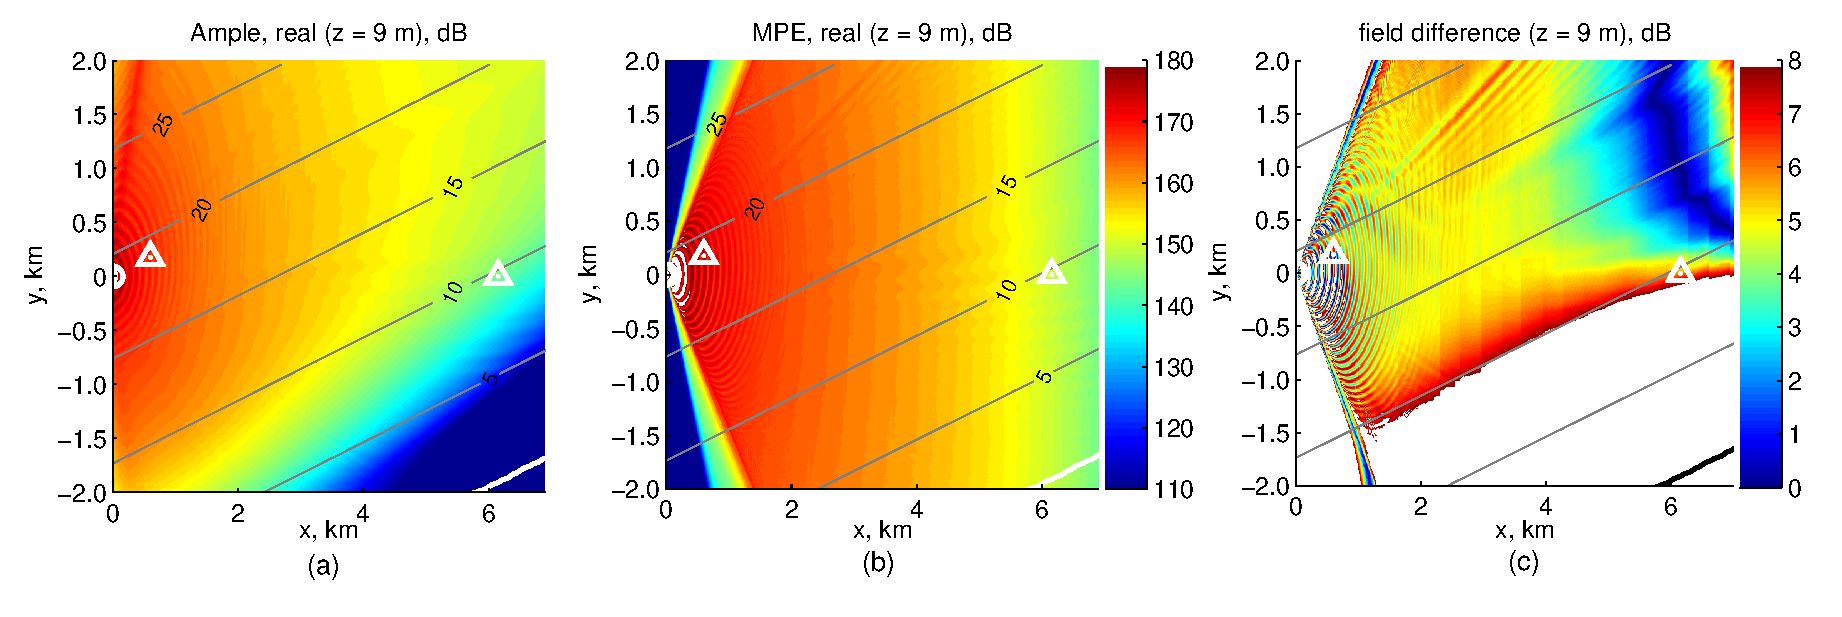
\includegraphics[width=0.9\textwidth]{images/seismo/pic_lineField.eps}
					\caption{Spatial distribution of the SEL parameter at a horizon of 9 m, calculated by Ample (\textbf{a}) and MPE (\textbf{b}) for the waveguide model with the bottom slope given by Equation~(\ref{m_polynom}). SEL difference modulus is also shown (\textbf{c}).}
					\label{fig4:scheme}
				\end{figure}
				
			\subsubsection{Realistic~Bathymetry}
				\par Let us now investigate the accuracy of SEL computations by the two models by using realistic bathymetry data in our geoacoustic waveguide model. In~this case we can also simulate the waveform of the signal at the point P2 and evaluate the accuracy of the model by a direct comparison with measurements~data.
				
				\par Figures~\ref{fig5:SEL}--\ref{fig7:waveform_and_spectra} show calculation results in the case of realistic bathymetry. Contour plots in Figure~\ref{fig5:SEL} show that SEL distribution patterns in this case are qualitatively similar to the ones obtained using a simplified bathymetry model \eqref{m_polynom}. Note that the difference between the two models (Figure~\ref{fig5:SEL}c) in this case also resembles the contour plot in Figure~\ref{fig4:scheme}c. SEL distributions clearly reflect bathymetry features in the area, and~their patterns show typical manifestation of the horizontal refraction in a shallow-water environment (noticeably greater field magnitude in the deeper part of the area).
			
				\begin{figure}[h]
					\centering
					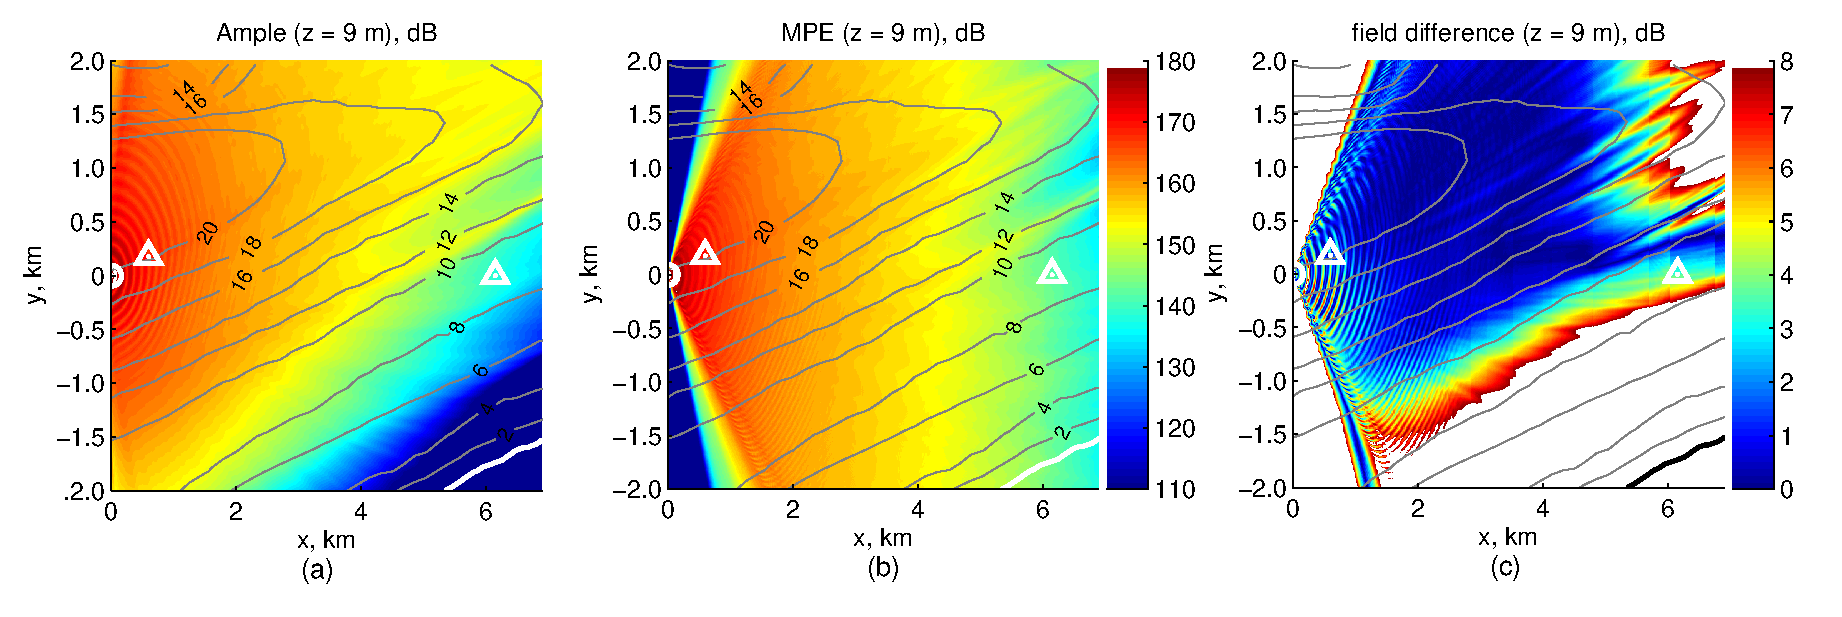
\includegraphics[width=0.9\textwidth]{images/seismo/pic_realField.eps}
					\caption{Spatial distribution of the SEL parameter at a horizon of 9 m, calculated by Ample (\textbf{a}) and MPE (\textbf{b}) for realistic bathymetry. Field difference module (\textbf{c}).}
					\label{fig5:SEL}
				\end{figure}
				
				\par Also note that the results obtained using Ample and MPE exhibit relatively good agreement along the path (i.e., along the line $y=0$) (see Figure~\ref{fig6:SEL} and also Figure~\ref{fig5:SEL}c along the $x$ axis). However, stepping aside from this line we observe significant differences in the results produced by the two models (see Figure~\ref{fig5:SEL}c). Clearly, this difference results from the limited aperture of the MPE in the horizontal plane, and~it is important to note that it reaches 8 dB even within the sector $\pm 3.5^\circ$ (about the line $y=0$) at the distance of ca. 7 km from the~source.
				
				\par A final validation of both models is accomplished by direct comparison of the pulse signal waveforms at the point P2 (recall that the source spectrum is reconstructed using the data from the point P1). This comparison in presented in Figure~\ref{fig7:waveform_and_spectra}). The~pulse obtained using Ample program exhibits significantly better agreement to the signal observed in the~experiment. 
				
				\par {Similar results were obtained for other recorders used in our measurements program, however, as~was mentioned earlier, we don not have the permission to present them in this publication. }
				
				\begin{figure}[h]
					\centering
					\includegraphics[width=0.9\textwidth]{images/seismo/pic_test_sel.eps}
					\caption{The dependence of the SEL on the range $x$ at the depth of 9 m calculated by Ample and MPE for realistic and linear~bathymetry.}
					\label{fig6:SEL}
				\end{figure}
				
				\begin{figure}[h]
					\centering
					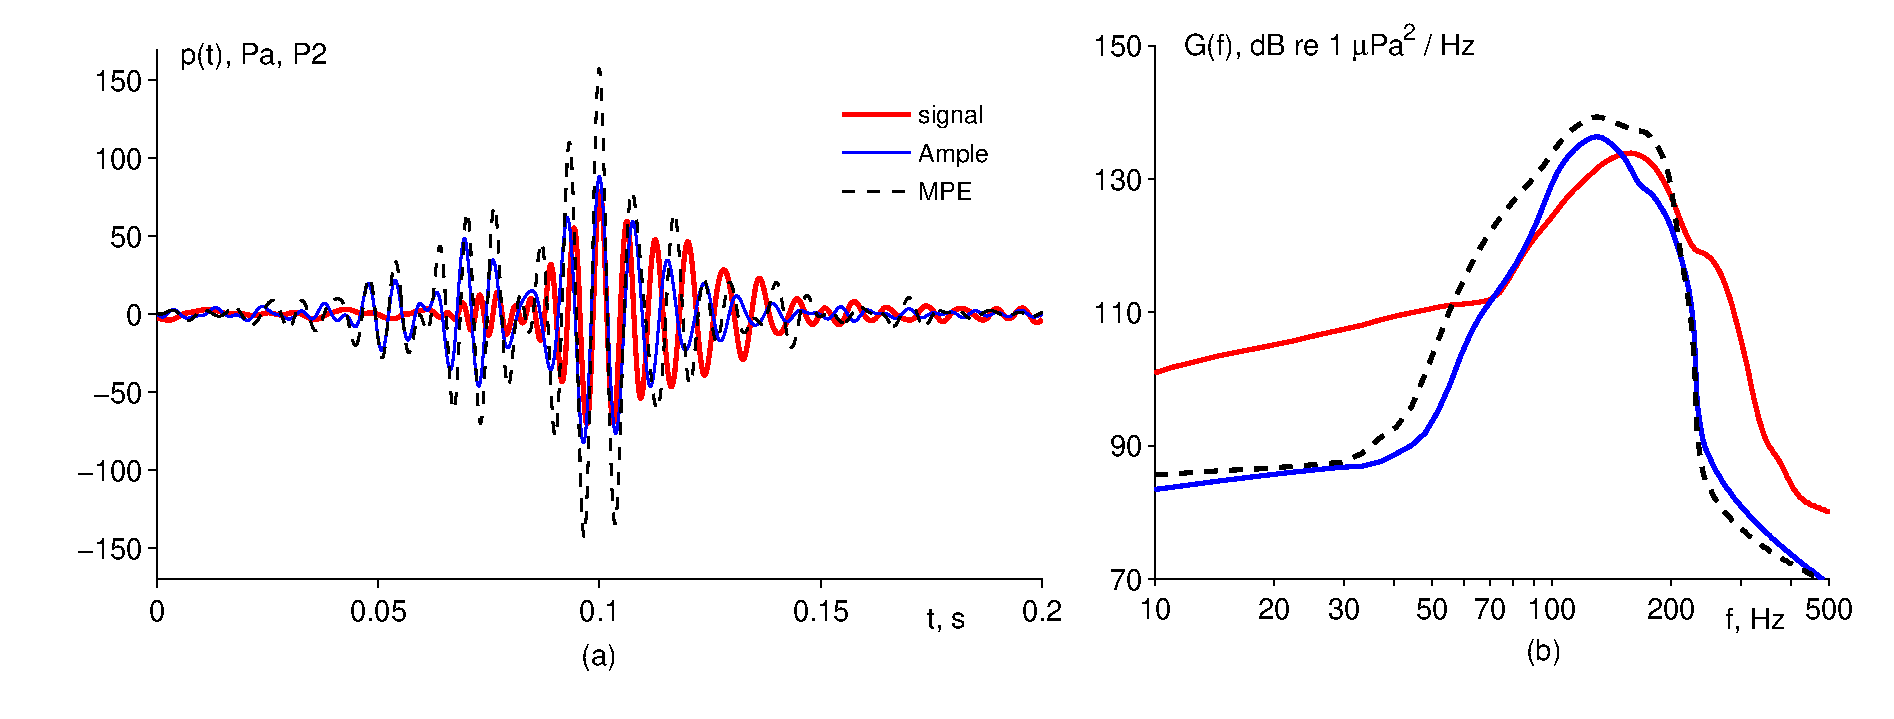
\includegraphics[width=0.9\textwidth]{images/seismo/pic_signal3.eps}
					\caption{Comparison of filtered experimental and model pulse signals at the reception point P2 (\textbf{a}) and their spectra (\textbf{b}).}
					\label{fig7:waveform_and_spectra}
				\end{figure}
			\subsubsection{Заключение}
				\par In this study we outlined and validated an algorithm for estimating SEL distribution over a large sea area in the course of acoustical monitoring of anthropogenic noises of various origins (e.g., pile driving and seismic survey). In~our algorithm, one recording unit (with a hydrophone) deployed in the area of interest is used for reconstructing effective source spectrum, and~the MPE theory is used for computing the field and SEL in the entire~area.
				
				\par The proposed approach is illustrated by using measurements data collected in the Sea of Okhotsk on the Sakhalin shelf. In~the considered setup, seismic pulses emitted by a survey vessel were recorded by the two receivers deployed near the vessel track. Pulses recorded by a receiver P1 located ca. 600 m from the emission point S were used for the source spectrum reconstruction, while the data from the other receiver P2 were used for the comparison with the simulation results and validation of the accuracy of SEL~modeling.
				
				\par It was shown that our approach allows to reproduce the pulse waveform at P2 with reasonable accuracy, both in time- and in frequency-domain. It is also important to note that pseudo-differential (wide-angle) adiabatic MPE produces significantly more accurate results than its narrow-angle counterpart, even if the mode interaction is taken into account. Despite the fact that total SEL of the signal in our simulation is reproduced with accuracy sufficient for practical applications (as we can from the direct comparison at the point P2), we still observe substantial disagreement of spectra for the frequency range 10--50 Hz (as can be seen from Figure~\ref{fig7:waveform_and_spectra}). This disagreement can be explained by the lack of knowledge about the layers constituting the sea bottom. It would be appropriate to incorporate a geoacoustic inversion algorithm into our software, so that the structure of bottom layers is also reconstructed on the basis of measurements data. Indeed, the~dispersion data of broadband seismic survey pulses obtained from acoustic measurements taken few kilometers away from the source (e.g., at~P2 in our case) can be used to perform the inversion by a warping-based method~\cite{bonnel2020}. This would further improve the quality of SEL distribution modeling. Of~course, even in this case the inverted parameters of the bottom layers would only be a path-averaged rough approximations to their counterparts in real marine environment, and~some important 3D effects arising from the variations of bottom parameters along and across the pass~\cite{lunkov2021} still would be~neglected.
				
				\par The question of choosing adequate mathematical methods for 3D modeling of sound propagation in cases when the computational cost is as important as the accuracy is still open. In~recent study~\cite{oliveira2021} a comprehensive comparison of several important approaches and respective computational codes was presented, and~it was shown that in many cases Gaussian beams~\cite{porter2019} can be an attractive option. In~our opinion however the advantages and shortcomings of the MPE-based technique are somewhat better balanced, though~some additional work still has to be done in order to include mode interaction~\cite{trofimov2015} into the model from~\cite{jsv}. 
\end{document}